%\documentclass[12pt]{beamer}
%\documentclass[ucs, handout]{beamer}

\documentclass[handout]{beamer}

\usetheme[numbers,totalnumbers,compress, nologo]{Statmod}
\usefonttheme[onlymath]{serif}
\setbeamertemplate{navigation symbols}{}

\mode<handout> {
	\usepackage{pgfpages}
	\setbeameroption{show notes}
	\pgfpagesuselayout{2 on 1}[a4paper, border shrink=5mm]
	\setbeamercolor{note page}{bg=white}
	\setbeamercolor{note title}{bg=gray!10}
	\setbeamercolor{note date}{fg=gray!10}
}

%\mode<presentation>
%{
%	\usetheme{Warsaw}
%	% or ...
%	
%	\setbeamercovered{transparent}
%	% or whatever (possibly just delete it)
%}


\usepackage[utf8]{inputenc}
\usepackage[T2A]{fontenc}
\usepackage[russian]{babel}
\usepackage{amsmath, amssymb}
\usepackage{booktabs}
\usepackage{graphicx}
\usepackage{multirow}
\usepackage{tikz}
\usepackage{ragged2e}

\setbeameroption{show notes}
\setbeamertemplate{headline}{}
%\setbeamertemplate{footline}{}
\setbeamertemplate{footline}{
	\leavevmode%
	\hbox{%
		\begin{beamercolorbox}[wd=.5\paperwidth,ht=2.5ex,dp=1.125ex,leftskip=.3cm plus1fill,rightskip=.3cm]{author in head/foot}%
			\usebeamerfont{author in head/foot}\insertsection
		\end{beamercolorbox}%
		\begin{beamercolorbox}[wd=.5\paperwidth,ht=2.5ex,dp=1.125ex,leftskip=.3cm,rightskip=.3cm plus1fil]{title in head/foot}%
			\usebeamerfont{title in head/foot}\hfill\insertframenumber\,/\,\inserttotalframenumber
	\end{beamercolorbox}}%
	\vskip0pt%
}


\title[Об мощности энергетического критерия]{Исследование эмпирической мощности энергетического критерия для проверки гипотезы о равенстве двух распределений.}
\author{Сивков Вячеслав, гр. 23.Б04-мм}
\institute{Санкт-Петербургский государственный университет\\
Кафедра статистического моделирования\\[0.03in]
Научный руководитель — д.ф.-м.н. \textbf{В. Б. Мелас}\\[0.1in]
Отчёт по производственной практике (научно-исследовательской работе)}

\date{  Санкт-Петербург\\ 2026г.}

\begin{document}

\begin{frame}
    \titlepage
    \note{
    Здравствуйте, уважаемые слушатели! Меня зовут Сивков Вячеслав. Вашему вниманию предлагается работа на тему: "Исследование асимптотической мощности энергетического критерия для проверки гипотезы о равенстве двух распределений в случае двух близких альтернатив". Работа выполнена на кафедре статистического моделирования СПбГУ под руководством доктора физико-математических наук, профессора Вячеслава Борисовича Меласа.
    }
\end{frame}

%\begin{frame}{Содержание}
%    \tableofcontents
%\end{frame}




\begin{frame}{Постановка задачи}
    \begin{block}{Задача}
        Проверка гипотезы о равенстве двух распределений:
        \[
        H_0: F_1 = F_2 \quad \text{против} \quad H_1: F_1 \neq F_2
        \]
    \end{block}
    
    \pause
    
    \begin{block}{Выборки}
        \begin{itemize}
            \item $X = (X_1, \ldots, X_n)$ из $F_1$
            \item $Y = (Y_1, \ldots, Y_m)$ из $F_2$
            \item Выборки независимые
        \end{itemize}
    \end{block}
    \note{
    В моей работе рассматривается классическая двухвыборочная задача: проверка гипотезы о том, что две независимые выборки $X$ и $Y$ извлечены из одного и того же распределения. Альтернатива состоит в том, что распределения не равны. Обозначим функции распределения $X_1$ и $Y_1$ через $F_1$ и $F_2$ соответственно.
    }
\end{frame}

\begin{frame}{Альтернативная гипотеза}
    \begin{block}{location-scale model}
        При $n = m$:
        \begin{align*}
        F_1(x) &= F(x) \\
        F_2(x) &= F\left(x \left(1 + \frac{h_2}{\sqrt{n}} \right) + \frac{h_1}{\sqrt{n}}\right)
        \end{align*}
    \end{block}
    
    \begin{itemize}
        \item $h_1$ --- параметр отличия по сдвигу
        \pause
        \item $h_2$ --- параметр отличия по масштабу
        \pause
        \item $F(x)$ --- базовое распределение
    \end{itemize}
    \note{
    	В данной работе внимание сосредоточено на важном частном случае: распределения отличаются лишь по сдвигу и/или масштабу. Различие описывается параметрами $h_1$ и  $h_2$, нормированными на корень из объема выборки. Здесь $h_1$ отвечает за отличие по сдвигу, $h_2$ — по масштабу, а $F(x)$ задает базовый вид распределения. Стоит отметить, что значительная часть широко известных тестов применяемых для проверки вышеуказанной гипотезы, в среднем, показывает себя хуже в ситуации когда имеется лишь отличие по масштабу, относительно случая когда есть различие по сдвигу. 
    	}
\end{frame}



\begin{frame}{Цели исследования}
    \begin{enumerate}
    	\item
        установить, насколько хорошо эмпирические мощности приближаются теоретическими при различных размерах выборки для некоторых базовых распределений,
        \pause
        \vspace{0.1in}
        \item
        провести сравнительный анализ эмпирических мощностей при различных значениях параметров $h_1$, $h_2$ и $n$,
        \pause
        \vspace{0.1in}
        \item
        исследовать влияние выбора функции $g(x)$ в энергетическом тесте на его мощность.
    \end{enumerate}
    \note{
    Основная цель исследования — проверить, насколько точно теоретические (асимптотические) значения мощности способны предсказывать реальную эмпирическую мощность энергетического теста на выборках разного объема. Также ставится задача провести сравнительный анализ поведения критерия при варьировании параметров сдвига и масштаба и изучить, как выбор ядерной функции $g(x)$ влияет на мощность.
    }
\end{frame}





\begin{frame}{Энергетический тест (ET)}
    \begin{block}{Статистика}
        \[
        \boxed{\Phi_{nm} = \Phi_{AB} - \Phi_A - \Phi_B}
        \]
        \begin{align*}
        \Phi_A &= \frac{1}{n^2} \sum_{1 \leq i \leq j \leq n} g(|X_i - X_j|) \\
        \Phi_B &= \frac{1}{m^2} \sum_{1 \leq i \leq j \leq m} g(|Y_i - Y_j|) \\
        \Phi_{AB} &= \frac{1}{nm} \sum_{i=1}^n \sum_{j=1}^m g(|X_i - Y_j|)
        \end{align*}
    \end{block}
    
    \begin{itemize}
        \item $g(x)$ --- монотонная и непрерывная функция
        \pause
        \item Используется статистика $n\Phi_{nn}$
    \end{itemize}
    \note{
    Объектом нашего внимания является энергетический тест. Его статистика $\Phi_{nm}$ основана на попарных расстояниях между элементами выборок, взвешенных некоторой монотонной непрерывной функцией $g(x)$. По сути, критерий измеряет "расстояние" между эмпирическими распределениями. В работе исследуется статистика вида $n\Phi_{nn}$ при равных объемах выборок. 
    }
\end{frame}




\begin{frame}{О вычислении асимптотической мощности энергетического теста}
	\begin{block}{Теорема, Мелас 2024}
		Пусть $g(x)$ монотонная (п.в.) дважды непрерывно дифференцируемая функция т.ч. $\mathbb{E}[g^2(\xi)] < \infty$\\
		\pause
		Тогда:\\
		Асимптотическая мощность теста $n\Phi_{nn}$ с уровнем значимости $\alpha$ равна
		\[ 
		1 - F \left(z_{1-\frac{\alpha}{2}} - \frac{b}{a} \right) + F \left(-z_{1-\frac{\alpha}{2}} - \frac{b}{a} \right),
		\]
		\pause
		где $F(t)$ --- функция стандартного нормального распределения, a $z_{1-\frac{\alpha}{2}}$ его $1-\frac{\alpha}{2}$ квантиль.
	\end{block}
	\note{
	Теоретическим фундаментом работы служит теорема Меласа, полученная в 2024 году. Она дает явную формулу для расчета асимптотической мощности энергетического теста через функцию стандартного нормального распределения и параметры $a$ и $b$, зависящие от базового распределения и функции $g(x)$. На практике возникает вопрос: насколько хорошее приближение дает эта предельная формула при различных объемах выборки? Можно ли использовать её как инструмент инженерного расчета мощности вместо долгих симуляций? Давайте обратимся к расчетам.
	}
\end{frame}


\begin{frame}
	
	\note{some text here}
\end{frame}



\begin{frame}{Стандартное нормальное распределение\\ Отличие по сдвигу}
\begin{table}[!h]
	\centering
	\caption{Значения эмпирической (EP) и асимптотической (AP) мощности ET ($h_2=0$, $g(x)=\ln(1+x^2)$)}
	\hspace*{-1.0cm}\begin{tabular}
		{lrrrrrrrrrr}
		\toprule
		& h1=1.0 & h1=2.0 & h1=3.0 & h1=4.0 & h1=5.0 & h1=6.0 \\
		\midrule
		EP (n=100) & 0.095 & 0.264 & 0.514 & 0.763 & 0.912 & 0.982 \\
		EP (n=400) & 0.093 & 0.259 & 0.506 & 0.761 & 0.915 & 0.983 \\
		EP (n=900) & 0.099 & 0.255 & 0.509 & 0.754 & 0.904 & 0.978\\
		EP (n=1600) & 0.086 & 0.245 & 0.497 & 0.751 & 0.919 & 0.983\\
		EP (n=2000) & 0.103 & 0.264 & 0.519 & 0.771 & 0.915 & 0.981\\
		EP (n=3000) & 0.111 & 0.275 & 0.529 & 0.767 & 0.917 & 0.983\\
		\addlinespace
		AP & 0.100 & 0.257 & 0.499 & 0.742 & 0.904 & 0.975 \\
		\bottomrule
	\end{tabular}
	\label{tbl:ap_normal_h1_diff}
\end{table}
\note{
На данном слайде представлены эмпирические мощности энергетического теста для стандартного нормального распределения при наличии только сдвига ($h_2=0$), где в качестве функции весов выбрана $g(x)=\ln(1+x^2)$. Сравнивая строчки эмпирической мощности (EP) при объемах от 100 до 3000 с нижней строкой асимптотической мощности (AP), мы наблюдаем довольно хорошую точность аппроксимации. Теоретическая формула дает крайне точное приближение реальной мощности, причем эта точность сохраняется даже на относительно малых выборках в 100 элементов.
}
\end{frame}

\begin{frame}{Стандартное нормальное распределение \\ Отличие по сдвигу}
	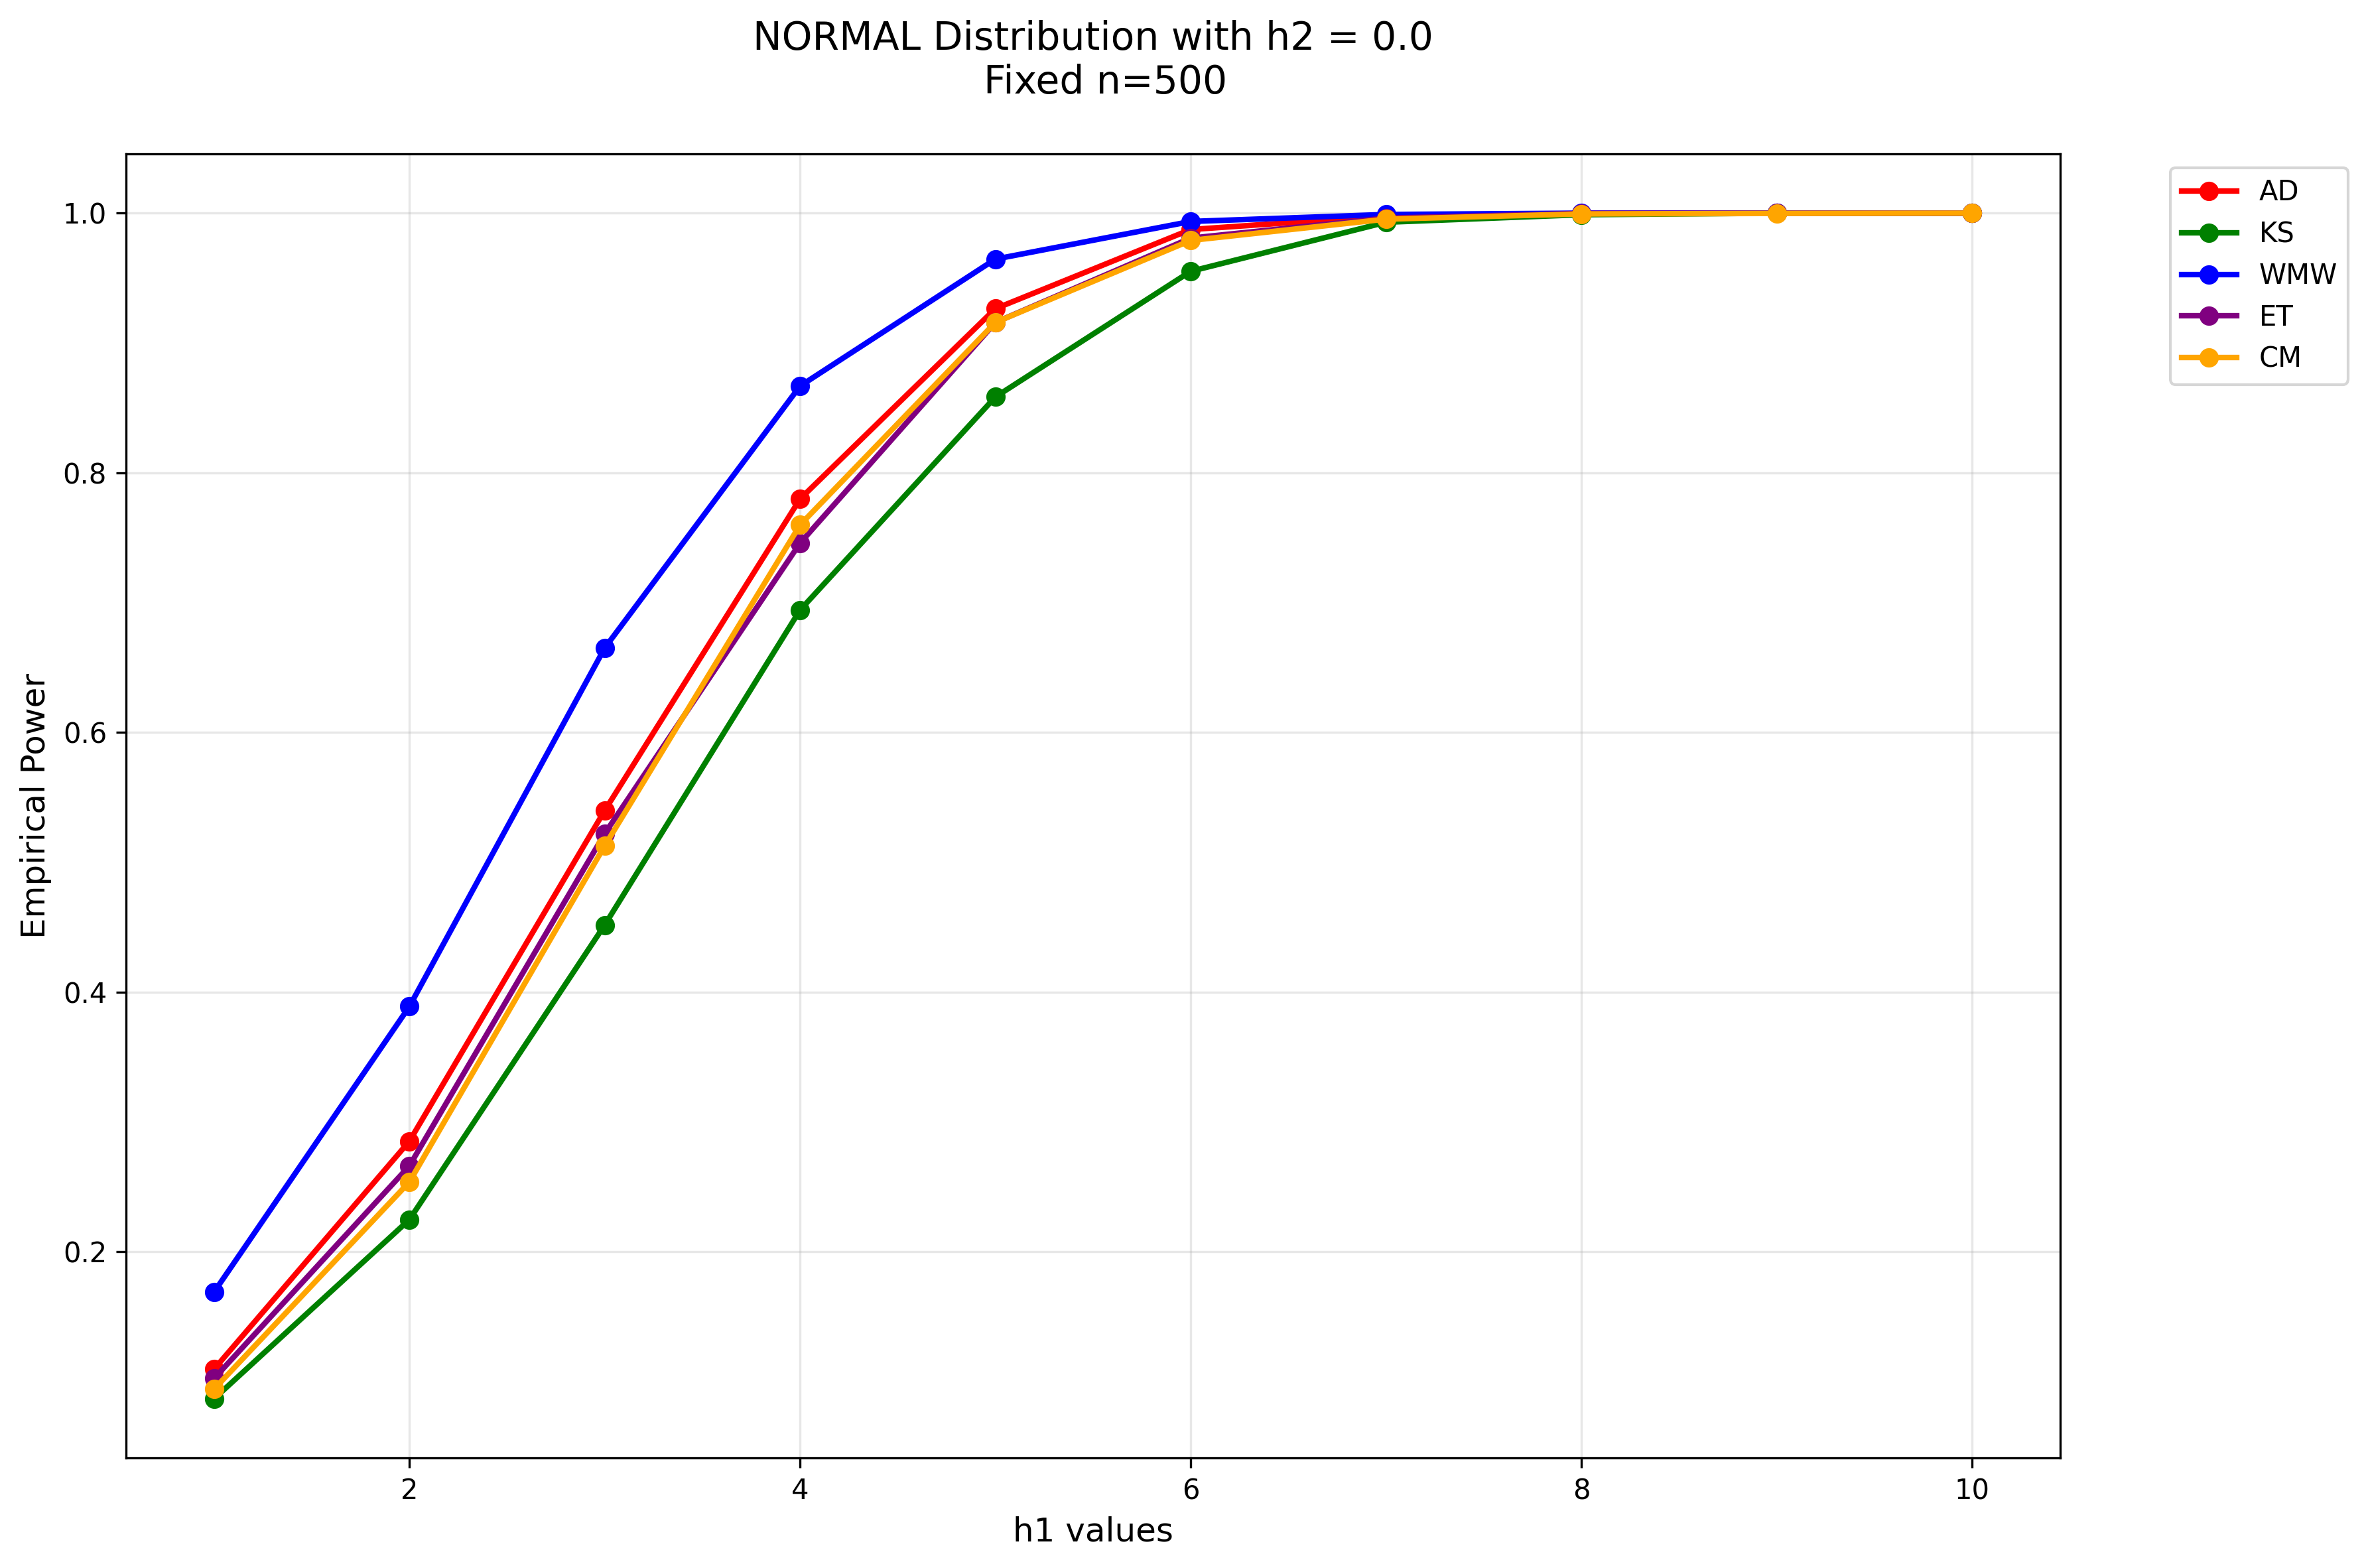
\includegraphics[width=0.9\textwidth]{pics/NORMAL_h2_n_EP (n_500).png}
	\note{На данном слайде представлены графики мощностей пяти тестов при изменении значения параметра отличия по сдвигу $h_1$ от $1$ до $10$ в случае стандартного нормального распределения при объеме выборки $n=500$. Видно, что наиболее мощным оказался тест WMW а наименее мощным тест KS.}
\end{frame}

\begin{frame}{Стандартное нормальное распределение \\ Отличие по масштабу}
	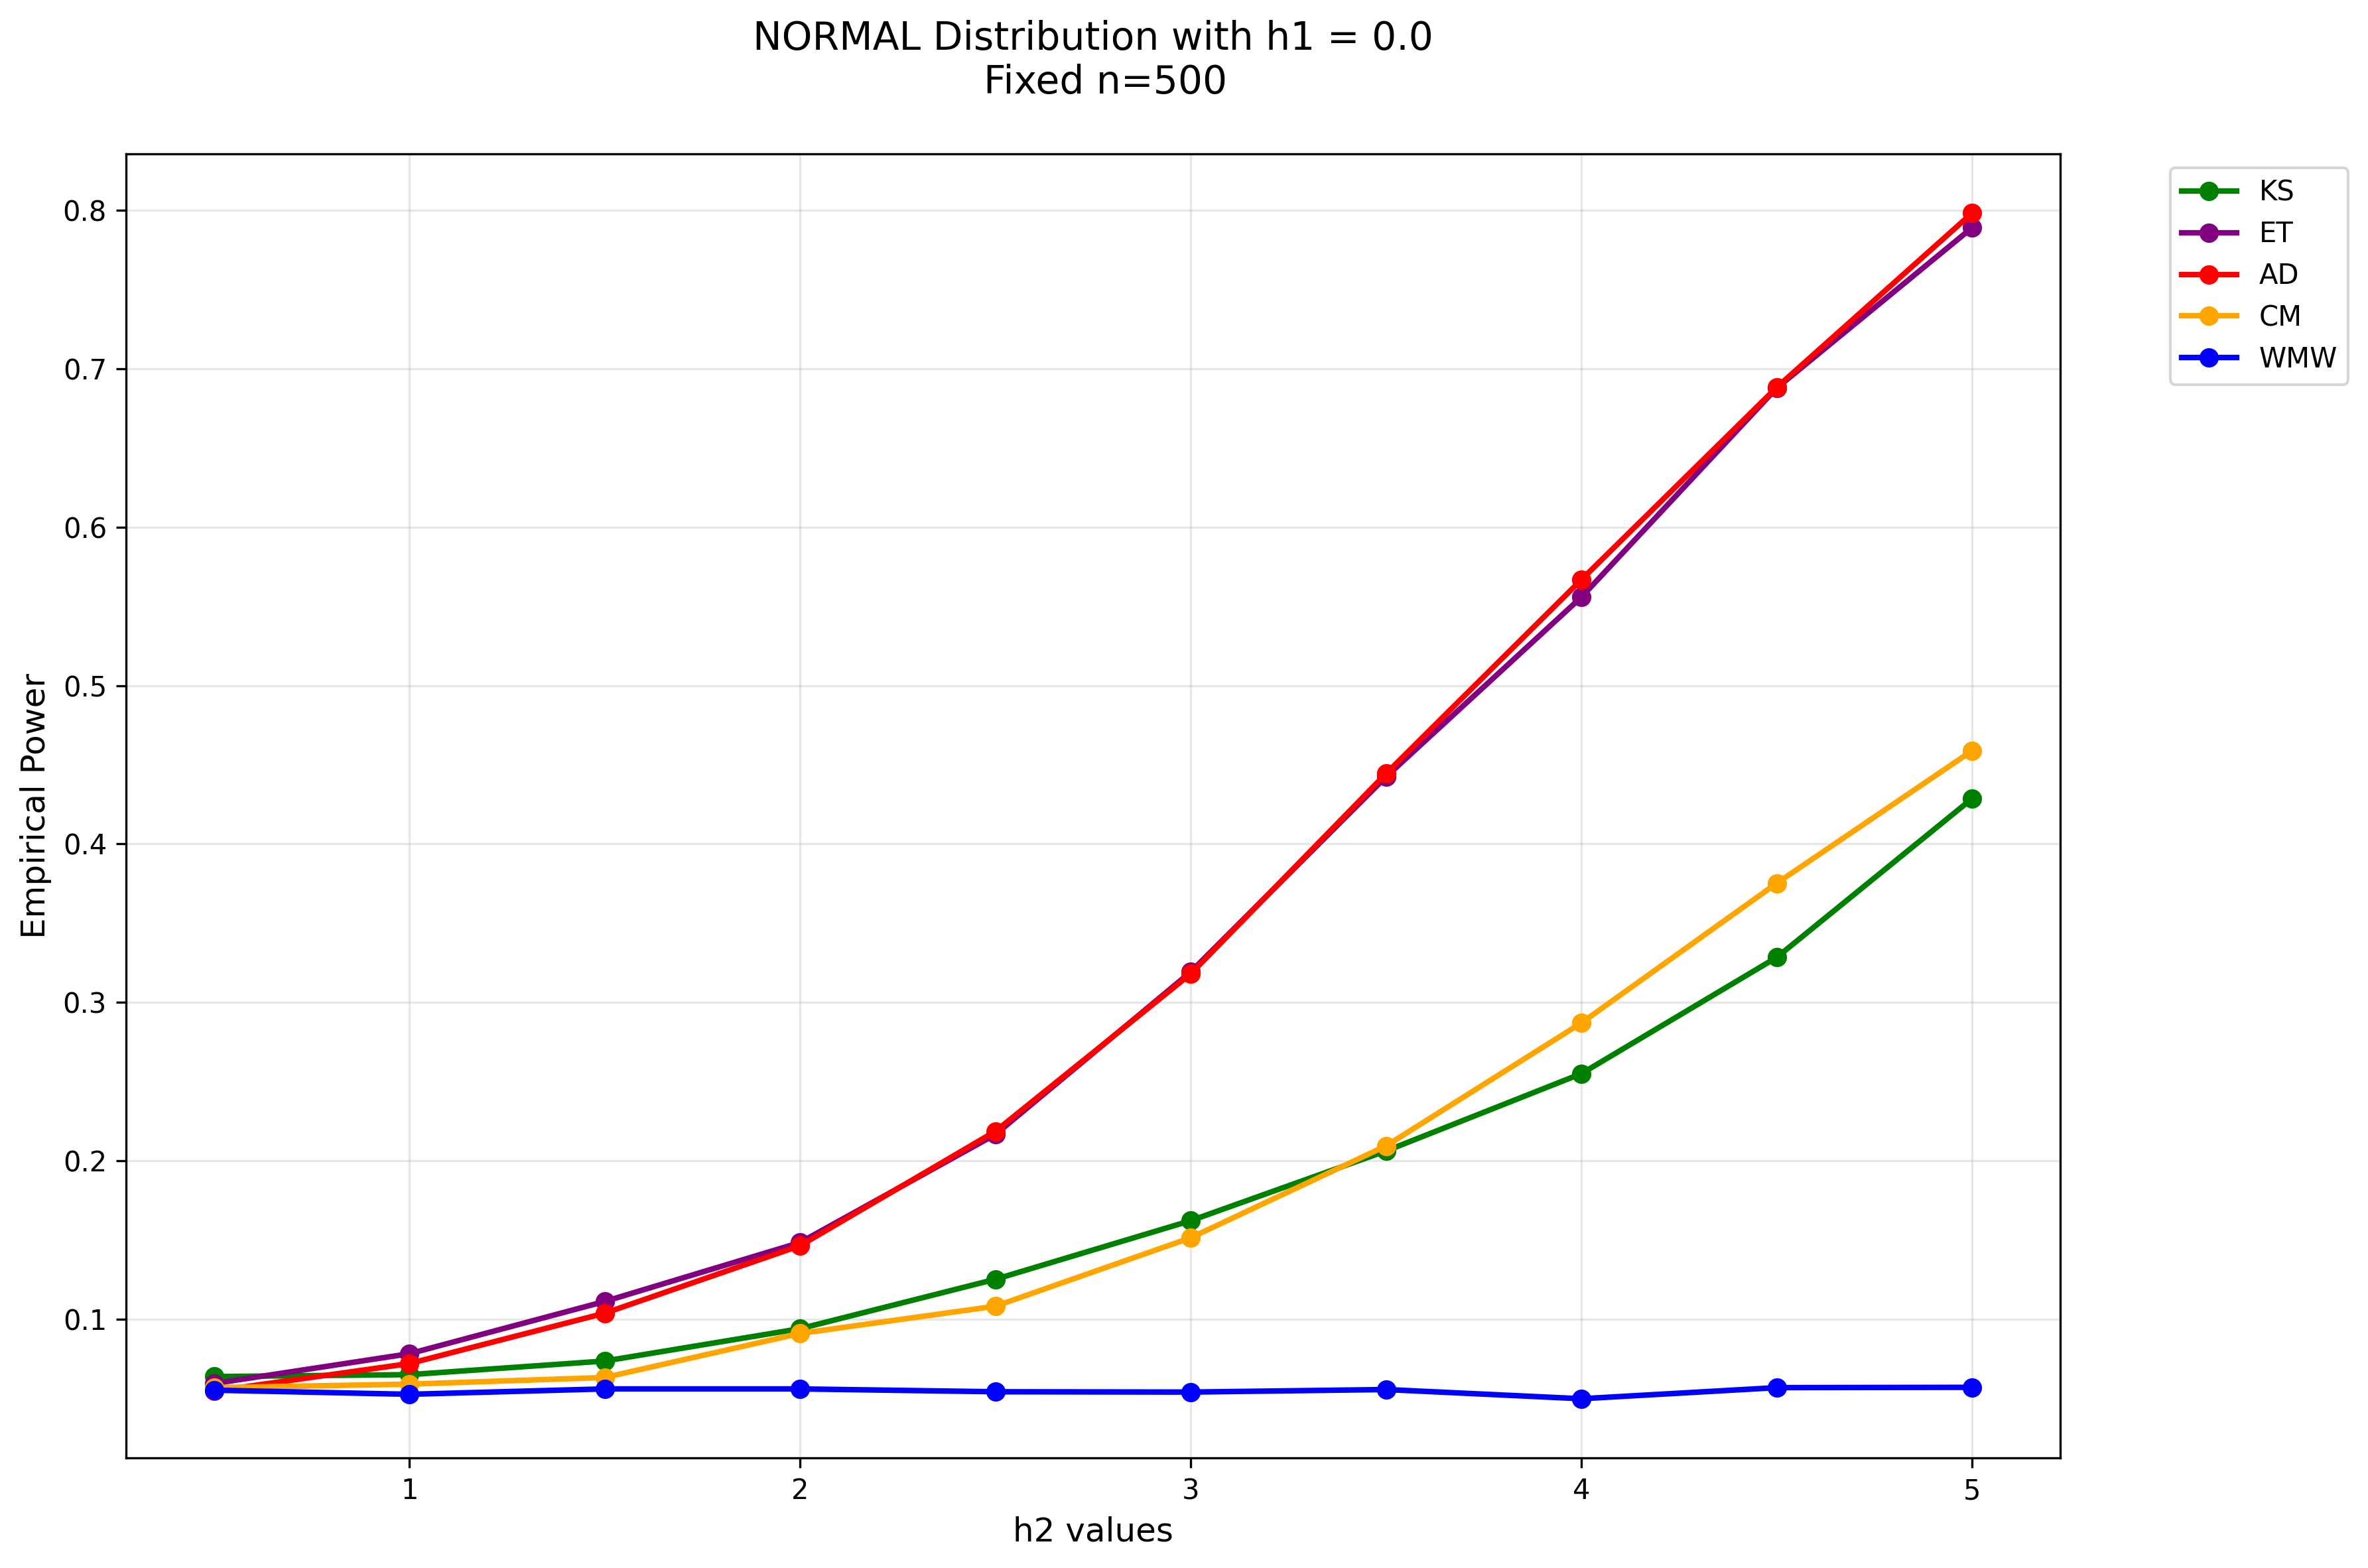
\includegraphics[width=0.9\textwidth]{pics/NORMAL_h1_n_EP (n_500).png}
	\note{На данном слайде представлены графики мощностей пяти тестов при изменении значения параметра отличия по масштабу $h_2$ от $0$ до $5$ в случае стандартного нормального распределения при объеме выборки $n=500$. Видно, что наиболее мощными оказались одновременно тесты AD и ET. А тест WMW в данной ситуации является бесполезным, так как его мощность примерно равна уровню значимости.}
\end{frame}




\begin{frame}{Стандартное распределение Коши \\ Отличие по масштабу}
	\begin{table}[!h]
		\caption{Значения эмпирической (EP) и асимптотической (AP) мощности ET ($h_1=0$, $g(x)=\ln(1+x^2)$)}
		\centering
		\hspace*{-1.0cm}\begin{tabular}
			{lrrrrrrrrrr}
			\toprule
			& h2=1.0 & h2=2.0 & h2=3.0 & h2=4.0 & h2=5.0 & h2=6.0\\
			\midrule
			EP (n=100) & 0.060 & 0.085 & 0.132 & 0.190 & 0.269 & 0.329 \\
			EP (n=400) & 0.063 & 0.109 & 0.167 & 0.257 & 0.370 & 0.509 \\
			EP (n=900) & 0.067 & 0.107 & 0.190 & 0.292 & 0.421 & 0.552 \\
			EP (n=1600) & 0.058 & 0.110 & 0.179 & 0.295 & 0.431 & 0.586 \\
			EP (n=2000) & 0.063 & 0.112 & 0.187 & 0.310 & 0.445 & 0.586 \\
			EP (n=3000) & 0.064 & 0.114 & 0.197 & 0.309 & 0.470 & 0.617 \\
			\addlinespace
			AP & 0.066 & 0.115 & 0.201 & 0.319 & 0.461 & 0.608 \\
			\bottomrule
		\end{tabular}
		\label{tbl:ap_cauchy_h2_diff}
	\end{table}
	\note{На данном слайде представлены результаты для стандартного распределения Коши при наличии только отличия по масштабу ($h_1=0$), где в качестве функции весов выбрана $g(x)=\ln(1+x^2)$. Видно, что при объёме выборки $n=3000$ погрешность аппроксимации не превышает значения $0.02$}
\end{frame}

\begin{frame}{Стандартное распределение Коши \\ Отличие по сдвигу}
	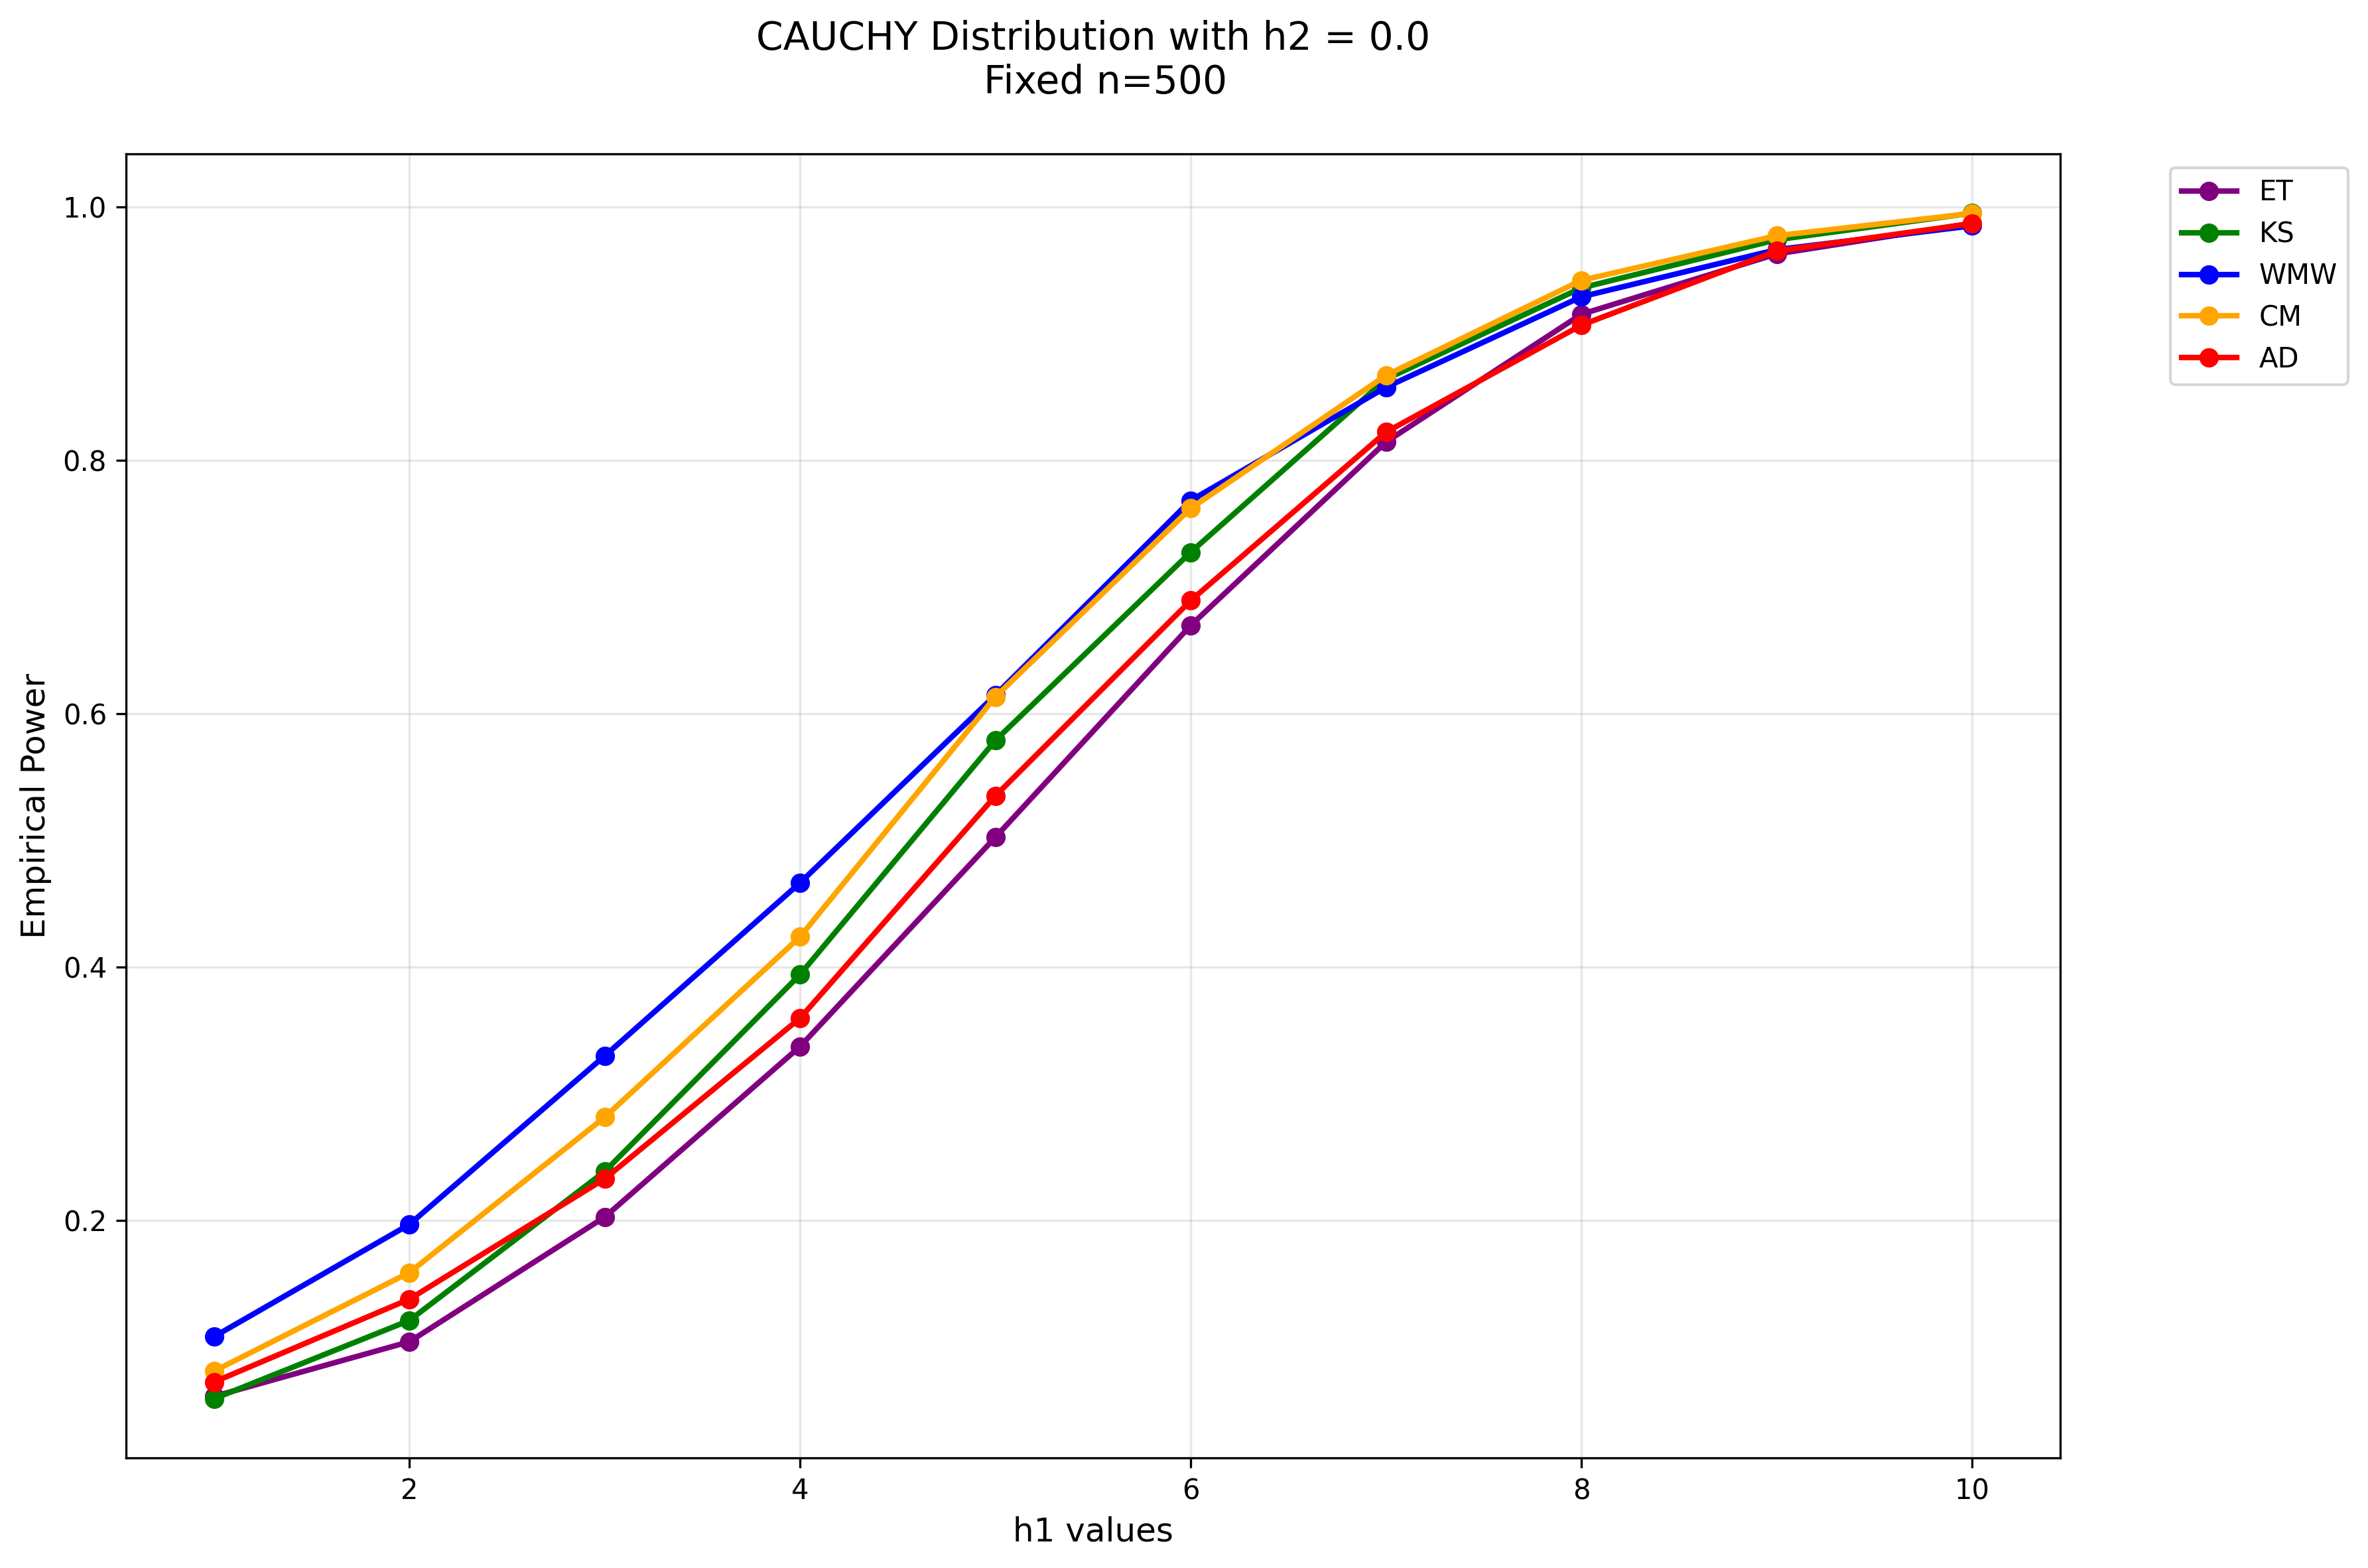
\includegraphics[width=0.9\textwidth]{pics/CAUCHY_h2_n_EP (n_500).png}
	\note{На данном слайде представлены графики мощностей пяти тестов при изменении значения параметра отличия по сдвигу $h_1$ от $1$ до $10$ в случае распределения Коши при объеме выборки $n=500$. Как и в предыдущем примере с отличием по сдвигу, в большинстве случаев наиболее мощным оказался тест WMW, а энергетический тест наоборот оказался наименее мощным.}
\end{frame}

\begin{frame}{Стандартное распределение Коши \\ Отличие по масштабу}
	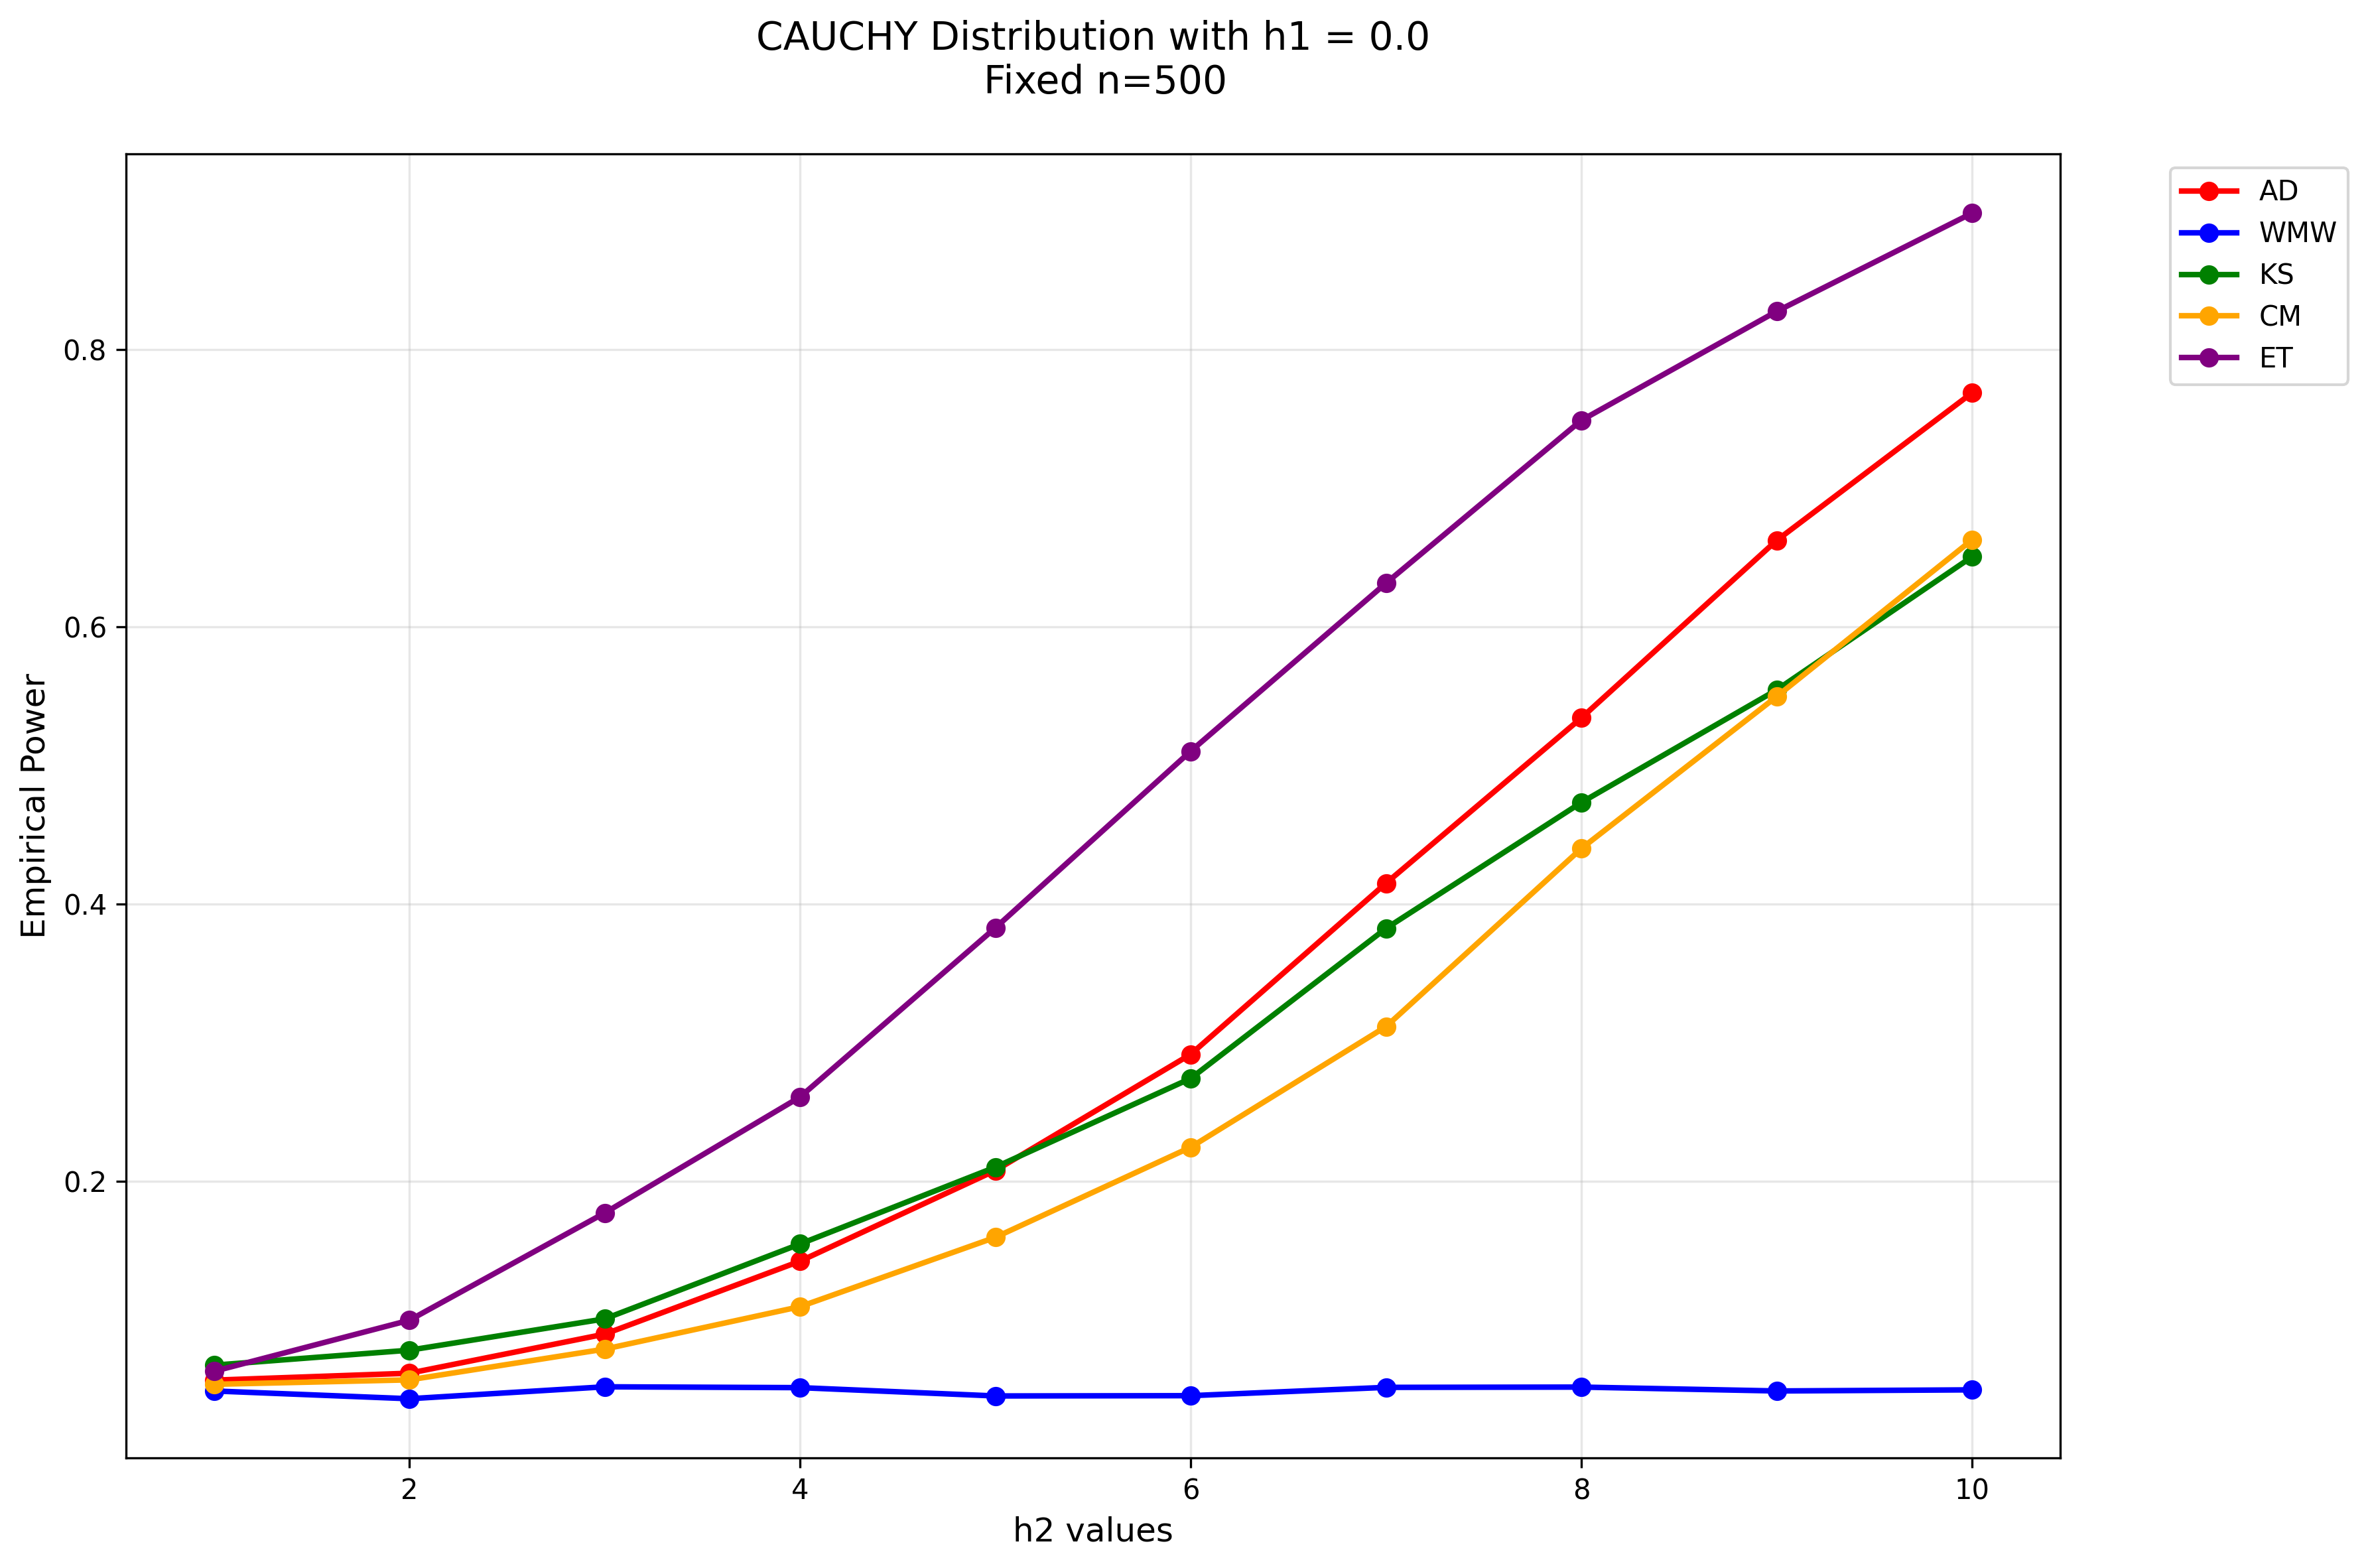
\includegraphics[width=0.9\textwidth]{pics/CAUCHY_h1_n_EP (n_500).png}
	\note{На данном слайде представлены графики мощностей пяти тестов при изменении значения параметра отличия по масштабу $h_2$ от $1$ до $10$ в случае распределения Коши при объеме выборки $n=500$.Здесь мы снова видим, что тест WMW является бесполезным. А энергетический тест выигрывает по мощности с заметным отличием.}
\end{frame}


\begin{frame}{Распределение Стьюдента ($\text{df}=20$)\\ Отличие по сдвигу}
\begin{table}[!h]
	\caption{Значения эмпирической (EP) и асимптотической (AP) мощности ($h_2=0$, $g(x)=\ln(1+x^2)$))}
	\centering
	\hspace*{-1.0cm}\begin{tabular}
		[t]{lrrrrrrrrrr}
		\toprule
		& h1=1.0 & h1=2.0 & h1=3.0 & h1=4.0 & h1=5.0 & h1=6.0 \\
		\midrule
		EP (n=100) & 0.105 & 0.264 & 0.495 & 0.749 & 0.903 & 0.978 \\
		EP (n=400) & 0.105 & 0.266 & 0.514 & 0.762 & 0.911 & 0.982\\
		EP (n=900) & 0.102 & 0.255 & 0.500 & 0.732 & 0.907 & 0.976\\
		EP (n=1600) & 0.110 & 0.255 & 0.511 & 0.758 & 0.906 & 0.979\\
		EP (n=2000) & 0.101 & 0.245 & 0.490 & 0.733 & 0.895 & 0.975\\
		
		EP (n=3000) & 0.094 & 0.251 & 0.480 & 0.744 & 0.888 & 0.977\\
		\addlinespace
		AP & 0.097 & 0.244 & 0.475 & 0.716 & 0.886 & 0.967 \\
		\bottomrule
	\end{tabular}
	\label{tbl:ap_student20_h1_diff}
\end{table}
\note{На данном слайде представлены результаты для распределения Стьюдента с 20-ю степенями свободы при наличии только отличия по сдвигу ($h_2=0$), где в качестве функции весов выбрана $g(x)=\ln(1+x^2)$. Видно, что при объёме выборки $n=3000$ погрешность аппроксимации не превышает значения $0.03$. Также, ожидаемо, результаты довольно близки к тому, что было рассмотрено в случае нормального распределения.}
\end{frame}


\begin{frame}{ Распределение Стьюдента \\ Отличие по сдвигу}
	\includegraphics[width=0.9\textwidth]{pics/STUDENT20_h2_n_EP (n_500).png}
	\note{На данном слайде представлены графики мощностей пяти тестов при изменении значения параметра отличия по сдвигу $h_1$ от $1$ до $10$ в случае распределения Стьюдента при объеме выборки $n=500$. Как и во всех предыдущих случаях с отличием по сдвигу, наиболее мощным оказывается тест WMW.}
\end{frame}

\begin{frame}{ Распределение Стьюдента \\ Отличие по масштабу}
	\includegraphics[width=0.9\textwidth]{pics/STUDENT20_h1_n_EP (n_500).png}
	\note{На данном слайде представлены графики мощностей пяти тестов при изменении значения параметра отличия по масштабу $h_2$ от $1$ до $10$ в случае распределения Стьюдента при объеме выборки $n=500$. Здесь мы снова видим, что тест WMW имеет мощность, примерно равную уровню значимости, и, следовательно, является почти бесполезным. Наиболее мощным оказался энергетический тест, сразу за ним расположился тест AD c небольшим отличием.}
\end{frame}






\begin{frame}{Два варианта ET}
	\begin{itemize}
	\item
	Далее, в таблицах, $\text{ET}_1$ обозначает энергетический 
	тест с $g_1(x) = \ln(1+x^2)$, а $\text{ET}_2$ обозначает энергетический тест с $g_2(x) = |x|$
	\pause
	\item
	Формула «не работает» для $g_2(x)$ в случае распределения Коши.
	\pause
	\item
	Но, если по ней посчитать, то AP$=0.05$
	\end{itemize}
	\note{Теперь посмотрим на то, как выбор функции $g$ влияет на мощность.
		  Заметим, что функция $g_2(x) = |x|$ не удовлетворяет условиям теоремы, но можно формально вычислить значение по формуле и сравнить с эмпирическими результатами.}
\end{frame}


\begin{frame}{А почему?}
	$$
	\int_{\mathbb{R}} \frac{ |x|^2 }{1+x^2} \ dx = ...
	$$
	\note{Краткая иллюстрация того, какое именно условие не выполняется.}
\end{frame}


\begin{frame}{Два варианта ET}
	\begin{table}[!h]
		\centering
		\caption{Стандартное нормальное распределение (h1=0)}
		\hspace*{-0.6cm}\begin{tabular}{l c c c c c c c c c c} 
			\toprule
			test & sample size & h2=1.0  & h2=2.0  & h2=3.0 & h2=4.0  & h2=5.0 \\ 
			\midrule
			\multirow{3}{*}{$\text{ET}_1$} 
			& n=100 & 0.05 & 0.09 & 0.1 & 0.33 & 0.49 \\ 
			& n=400 & 0.06& 0.13 & 0.27& 0.51  & 0.74 \\ 
			& n=900 & 0.07 & 0.16  & 0.34 & 0.59 & 0.82 \\ 
			\addlinespace
			\addlinespace
			\multirow{3}{*}{$\text{ET}_2$} 
			& n=100 & 0.05  & 0.08 & 0.15 & 0.27  & 0.42 \\ 
			& n=400 & 0.05  & 0.09  & 0.2  & 0.38  & 0.62 \\ 
			& n=900 & 0.06  & 0.11  & 0.23 & 0.45 & 0.7 \\ 
			\bottomrule
		\end{tabular}
		\label{tbl:et_comp_normal_h2}
	\end{table}
	\note{На данном слайде представлены эмпирические мощности в случае стандартного нормального распределения для двух различных ядерных функций. Видно, что при $g(x)=|x|$ мощность в большинстве случаев оказывается ниже чем при использовании $g(x)=\ln(1+x^2)$}
\end{frame}


\begin{frame}{Два варианта ET}
	%aboba
	% Table for CAUCHY_h2
	\begin{table}[!h]
		\centering
		\caption{Стандартное распределение Коши (h2=0)}
		\hspace*{-0.6cm}\begin{tabular}{l c c c c c c c c c c} 
			\toprule
			test & sample size & h1=1.0 & h1=2.0 & h1=3.0 & h1=4.0 & h1=5.0 \\ 
			\midrule
			\multirow{3}{*}{$\text{ET}_1$} 
			& n=100 & 0.08 & 0.11 & 0.21 & 0.35 & 0.52 \\ 
			& n=400 & 0.06 & 0.11 & 0.21 & 0.34 & 0.52 \\ 
			& n=900 & 0.07 & 0.12 & 0.22 & 0.36 & 0.53 \\ 
			\addlinespace
			\addlinespace
			\multirow{3}{*}{$\text{ET}_2$} 
			& n=100 & 0.06 & 0.07 & 0.07 & 0.07 & 0.08  \\ 
			& n=400 & 0.05 & 0.05 & 0.05 & 0.06 & 0.06 \\ 
			& n=900 & 0.04 & 0.05 & 0.05 & 0.05 & 0.06 \\ 
			\bottomrule
		\end{tabular}
		\label{tbl:et_comp_cauchy_h1}
	\end{table}
	\note{На данном слайде представлены эмпирические мощности в случае стандартного распределения Коши для двух различных ядерных функций. Видно, что при $g(x)=|x|$ мощность оказывается ниже чем при использовании $g(x)=\ln(1+x^2)$ и примерно равна значению AP которое в свою очередь примерно равно уровню значимости.}
\end{frame}





\begin{frame}{Выводы}
    \begin{enumerate}
        \item \textbf{Аппроксимация:}
        \begin{itemize}
        \item
        В случае нормального распределения эмпирические мощности отличаются от асимптотических не более чем на $0.1$.
    	\end{itemize}
		\pause
        \item \textbf{Мощность тестов зависит от типа отличия:}
        \begin{itemize}
            \item Отличие по масштабу: чаще всего ET наиболее мощный.
            \item В случае отличия по сдвигу, чаще всего наиболее мощным оказывается WMW
        \end{itemize}
       
    \end{enumerate}
    \note{После проделанной работы можно сделать следующие выводы:
    	 В случае нормального распределения эмпирические мощности отличаются от асимптотических не более чем на $0.1$.
    	 
    	 В случае отличия по масштабу, чаще всего наиболее мощным оказывается энергетический тест. Причём все остальные тесты (за исключением AD) заметно менее мощные в этом случае для всех рассмотренных распределений.
    	 В случае отличия по сдвигу, чаще всего наиболее мощным оказывается тест WMW
    	 
    	 }
\end{frame}

\begin{frame}{Выводы}
    \begin{block}{Выполненная работа}
        \begin{itemize}
            \item Проведено сравнение мощностей пяти статистических тестов
            \item Изучено качество приближения эмпирических мощностей асимптотическими
            \item Проанализировано влияние типа отличия распределений
        \end{itemize}
    \end{block}
    \pause
    \begin{block}{Дальнейшая работа}
        \begin{itemize}
            \item Исследовать асимптотические мощности для более широкого класса функций $g(x)$
        \end{itemize}
    \end{block}
    \note{Все поставленные в начале исследования задачи были выполнены. 
    	  Стоит отметить, что можно попытаться исследовать мощности для более широкого класса ядерных функций. }
\end{frame}


\begin{frame}{Литература}
    \begin{thebibliography}{9}
    \bibitem{melas2024}
    В. Б. Мелас, Д. И. Сальников.
    \textit{Об асимптотической мощности «энергетического» теста для проверки гипотез о равенстве двух распределений}.
    Вестник СПбГУ. Математика. Механика. Астрономия, 2024.
    
    \bibitem{AD_article}
    F.-W. Scholz, M. A. Stephens.
    \textit{K-Sample Anderson–Darling Tests}.
    Journal of the American Statistical Association, 1987.
    
    \bibitem{WMW_article}
    H. B. Mann, D. R. Whitney.
    \textit{On a Test of Whether one of Two Random Variables is Stochastically Larger than the Other}.
    Annals of Mathematical Statistics, 1947.
    
    \bibitem{KS_CM_article}
    H. Buning.
    \textit{Kolmogorov-Smirnov and Cramér-von Mises Type Two-Sample Tests with Various Weight Functions}.
    Communications in Statistics - Simulation and Computation, 2001.
    \end{thebibliography}
    \note{На этом слайде представлен список источников.}
\end{frame}


\begin{frame}
	\begin{center}
		Fin.
	\end{center}
	\note{На этом мой доклад окончен. Благодарю за внимание.}
\end{frame}



\begin{frame}{Обозначения}
	\begin{itemize}
		\item
		Пусть $f(x)$ обозначает плотность $F_1$
	\end{itemize}
\end{frame}

\begin{frame}{Обозначения}
	
	\begin{align*}
		J_1 &= \mathbb{E}[g(\xi - \eta)]\\
		\pause
		J_2 &= \mathbb{E}[g^2(\xi - \eta)] \\
		\pause
		J_3 &= \mathbb{E}[g(\xi - \eta)g(\eta - \gamma)] \\[0.2in]
		\pause
		J^*_1(h_1) &= \frac{1}{2}h^2_1 \int_{\mathbb{R}^2} g''(x-y)f(x)f(y)dxdy \\
		\pause
		J^*_2(h_2) &= \frac{1}{2}h^2_2 \int_{\mathbb{R}^2} (y^2-\frac{(x-y)^2}{2})g''(x-y)f(x)f(y)dxdy \\
	\end{align*}
	
\end{frame}

\begin{frame}{Обозначения}
	
	\begin{align*}
		&b^2_1 = | J^*_1(h_1) |\\
		\pause
		&b^2_2 = | J^*_2(h_2) |\\
		\pause
		&b = \sqrt{b^2_1 + b^2_2} \\
		\pause
		&a^2 = \sqrt{ J_2 + J^2_1 - 2J_3}
	\end{align*}
	
\end{frame}

\begin{frame}{Тест Андерсона-Дарлинга (AD)}
	    \begin{block}{Статистика для k выборок}
		        \[
		        A_{kN}^2 = \frac{1}{N} \sum_{i=1}^k \frac{1}{n_i} \sum_{j=1}^{N-1} \frac{(NM_{ij} - jn_i)^2}{j(N-j)}
		      \]
		    \end{block}
	    
	    \begin{itemize}
		        \item $N = n_1 + \ldots + n_k$ - общий объем выборок
		        \item $M_{ij}$ - количество элементов i-й выборки $\leq Z_{(j)}$
		        \item $Z_{(1)}, \ldots, Z_{(N)}$ - вариационный ряд
		    \end{itemize}
	    \end{frame}



\begin{frame}{Тест Колмогорова-Смирнова (KS)}
	    \begin{block}{Статистика}
		        \[
		        KS = \max_{1 \leq i \leq N} |\hat{F}(Z_{(i)}) - \hat{G}(Z_{(i)})|
		        \]
		    \end{block}
	    
	    \begin{itemize}
		        \item $\hat{F}$, $\hat{G}$ - эмпирические функции распределения
		        \item $Z_{(1)}, \ldots, Z_{(N)}$ - объединенный вариационный ряд
		        \item $N = n + m$
		    \end{itemize}
	\end{frame}



\begin{frame}{Тест Крамера-фон Мизеса (CM)}
	    \begin{block}{Статистика}
		        \[
		        CM = \frac{mn}{N^2} \sum_{i=1}^N (\hat{F}(Z_{(i)}) - \hat{G}(Z_{(i)}))^2
		        \]
		    \end{block}
	    
	\end{frame}



\begin{frame}{Тест Вилкоксона-Манна-Уитни (WMW)}
	    \begin{block}{Статистика}
		        \[
		        U_{nm} = \sum_{i=1}^n \sum_{j=1}^m \chi(X_i, Y_j)
		        \]
		        \[
		        \chi(X_i, Y_j) = 
		        \begin{cases}
			        1, & X_i \geq Y_j \\
			        0, & X_i < Y_j
			        \end{cases}
		        \]
		    \end{block}
	    
	    \begin{itemize}
		        \item Чувствителен к сдвигу распределений
		    \end{itemize}
	\end{frame}

\begin{frame}{Вычисление критического значения}
	\begin{enumerate}
		\item Генерируем выборки $X^{(k)}$ и $Y^{(k)}$ размера $n$, из $F_1$, где $k \in \overline{1,\ldots, M}$.
		\pause
		\item Вычисляем $T(X^{(k)}, Y^{(k)})$ для всех $k \in \overline{1,\ldots, M}$
		\pause
		\item Получаем выборку из распределения $T(X,Y)$ размера $M$, по ней строим эмпирическое распределение $\hat{T}(X,Y)$.
		\pause
		\item В качестве $c_{\alpha}$ берём $1 - \alpha$ квантиль $\hat{T}(X,Y)$.
	\end{enumerate}
\end{frame}


\begin{frame}{Вычисление эмпирической мощности}
	\begin{enumerate}
		\item Генерируем $X^{(i)}, Y^{(i)}$ -- выборки размера $n$ из $F_1$ и $F_2$ соответственно, для $i \in \overline{1,\ldots, N}$.
		\pause
		\item Считаем количество отвержений $H_0$ как $cnt =  \#\{ (X^{(i)},Y^{(i)}) \ | \ T(X^{(i)}, Y^{(i)}) \geqslant c_{\alpha}, \ i \in \overline{1,\ldots, N} \}$.
		\pause
		\item В качестве эмпирической мощности берём $ \frac{cnt}{N}$.
	\end{enumerate}
\end{frame}


\end{document}